\section{Конструкторская часть}

\subsection{Графовое представление мульти-генома}

Рассмотрим множество $ \{\Gamma_1,\Gamma_2,\ldots,\Gamma_m\} $ последовательностей ДНК $ \Gamma_i $ организмы-носители которых принадлежат одному виду, называемое мульти-геномом\cite{15_brandenburger2018multi,16_zekic2018pan}. Мы предлагаем рассмотреть расширенную модель графа де Брюйна $ B\left(\{\Gamma_1,\Gamma_2,\ldots,\Gamma_m\},\ \Sigma_{DNA}, \ k\right)=G\left(V,E\right) $, где каждый узел $ v \in V $ дополнен информацией о том, каким геномам он принадлежит. Так, каждый геном $ \Gamma_i $ представляет собой путь в графе $ B\left(\{\Gamma_1,\Gamma_2,\ldots,\Gamma_m\},\ \Sigma_{DNA},\ k\right) $. 

Рассмотрим теперь Марковскую цепь, образованную\cite{17_heath2021computing} описанной структурой графа де Брюйна $ B\left(\{\Gamma_1,\Gamma_2,\ldots,\Gamma_m\},\ \Sigma_{DNA}, k\right) $. Расценивая индексы строки ДНК в качестве дискретных моментов времени, пространство состояний для такой Марковской цепи будет $ V $. Дополним каждое ребро $ \left(u,v\right) \in E $ значением $ p_{uv} $, которое выражает вероятность наблюдения нуклеотида $ v\left[k-1\right] $, следующего за к-мерой $ u $ в мульти-геноме вида. 

Обозначим предложенную графовую модель $ MBG\left(\{\Gamma_1,\Gamma_2,\ldots,\Gamma_m\},\ \Sigma_{DNA},\ k\right) $. Для каждой последовательности нуклеотидов $ H $ может быть посчитана вероятность $ p_H $ обнаружения этой последовательности в мульти-геноме вида как произведение весов ребер, составляющих путь в $ MBG\left(\{\Gamma_1,\Gamma_2,\ldots,\Gamma_m\},\ \Sigma_{DNA},\ k\right) $.

\subsection{Формализация геномных вариаций}
Концепция пузырей (bubbles) предложена\cite{18_minkin2020applications,19_dabbaghie2021bubblegun} для описания геномных вариаций между гомологичными последовательностями. В данной работе термины \textit{вариация нуклеотида} (\textit{single-nucleotide variation}) and \textit{точечная мутация} (\textit{point mutation}) использованы взаимозаменяемо, оба термина относятся к единичному различию между последовательностями нуклеотидов. Обнаружение и подсчет единичных вариаций нуклеотидов позволит в дальнейшем рассчитать оценку гомологичности для подпоследовательностей. 

Пузырь -- это подграф, соответсвующий возможной мутации\cite{18_minkin2020applications}. Пара путей в графе $ x $ и $ y $ образуют пузырь $ \left(x,y\right) $, если выполняются следующие условия:
\begin{itemize} 
	\item $ x $ и $ y $ имеют общие начальные и конечные вершины;
	\item $ x $ и $ y $ не имеют никаких других общих вершин, кроме начальных и конечных.
\end{itemize}

Примеры пузырей, относящихся к различным типам точечных мутаций продемонстрированы на рисунке \ref{fig:pm_ex}.
\begin{figure*}[!th]
	\centering
	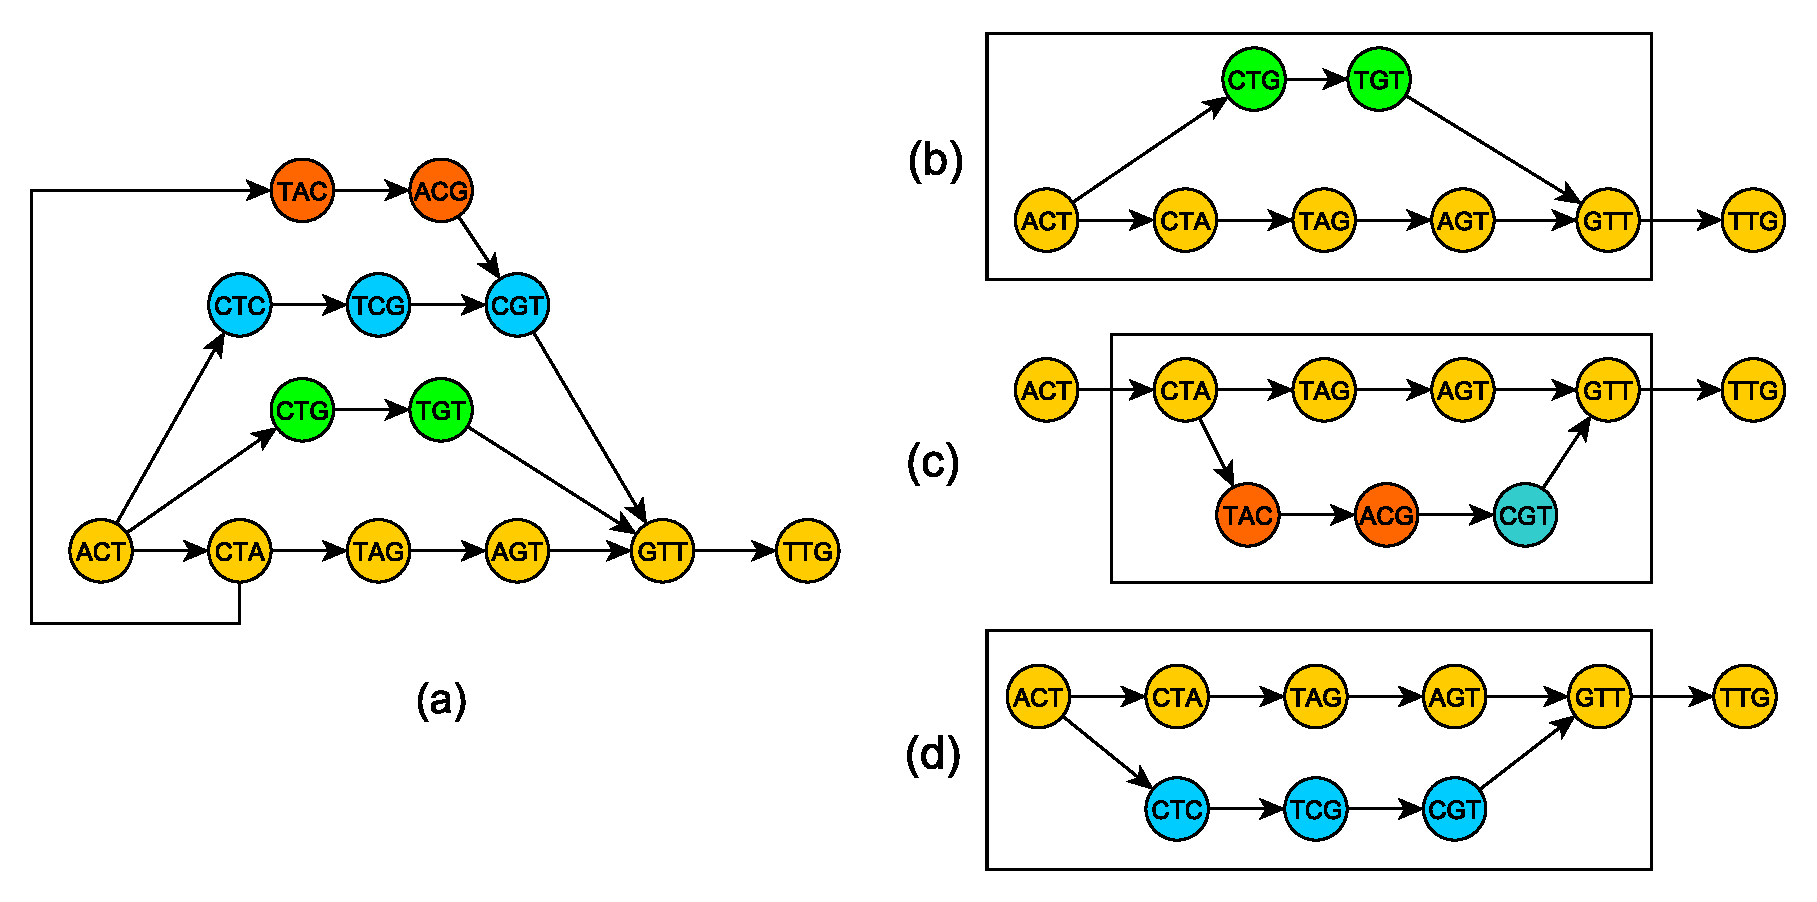
\includegraphics[width=0.8\textwidth]{img/pm_ex.pdf}
	\caption{Пузыри, образованные точечными мутациями разных типов: (a) подграф, содержащий пути, соответсвующие гомологичным последовательностям; (b) пузырь, соответствующий удалению нуклеотида; (c) пузырь, соответствующий вставке нуклеотида; (d) пузырь, соответствующий замене нуклеотида.}
	\label{fig:pm_ex}
\end{figure*}

Несколько точечных мутаций могут образовать пузырь больших размеров -- сложный пузырь -- как показано на рисунке \ref{fig:cv_ex}. 
\begin{figure*}[h!t]
	\centering
	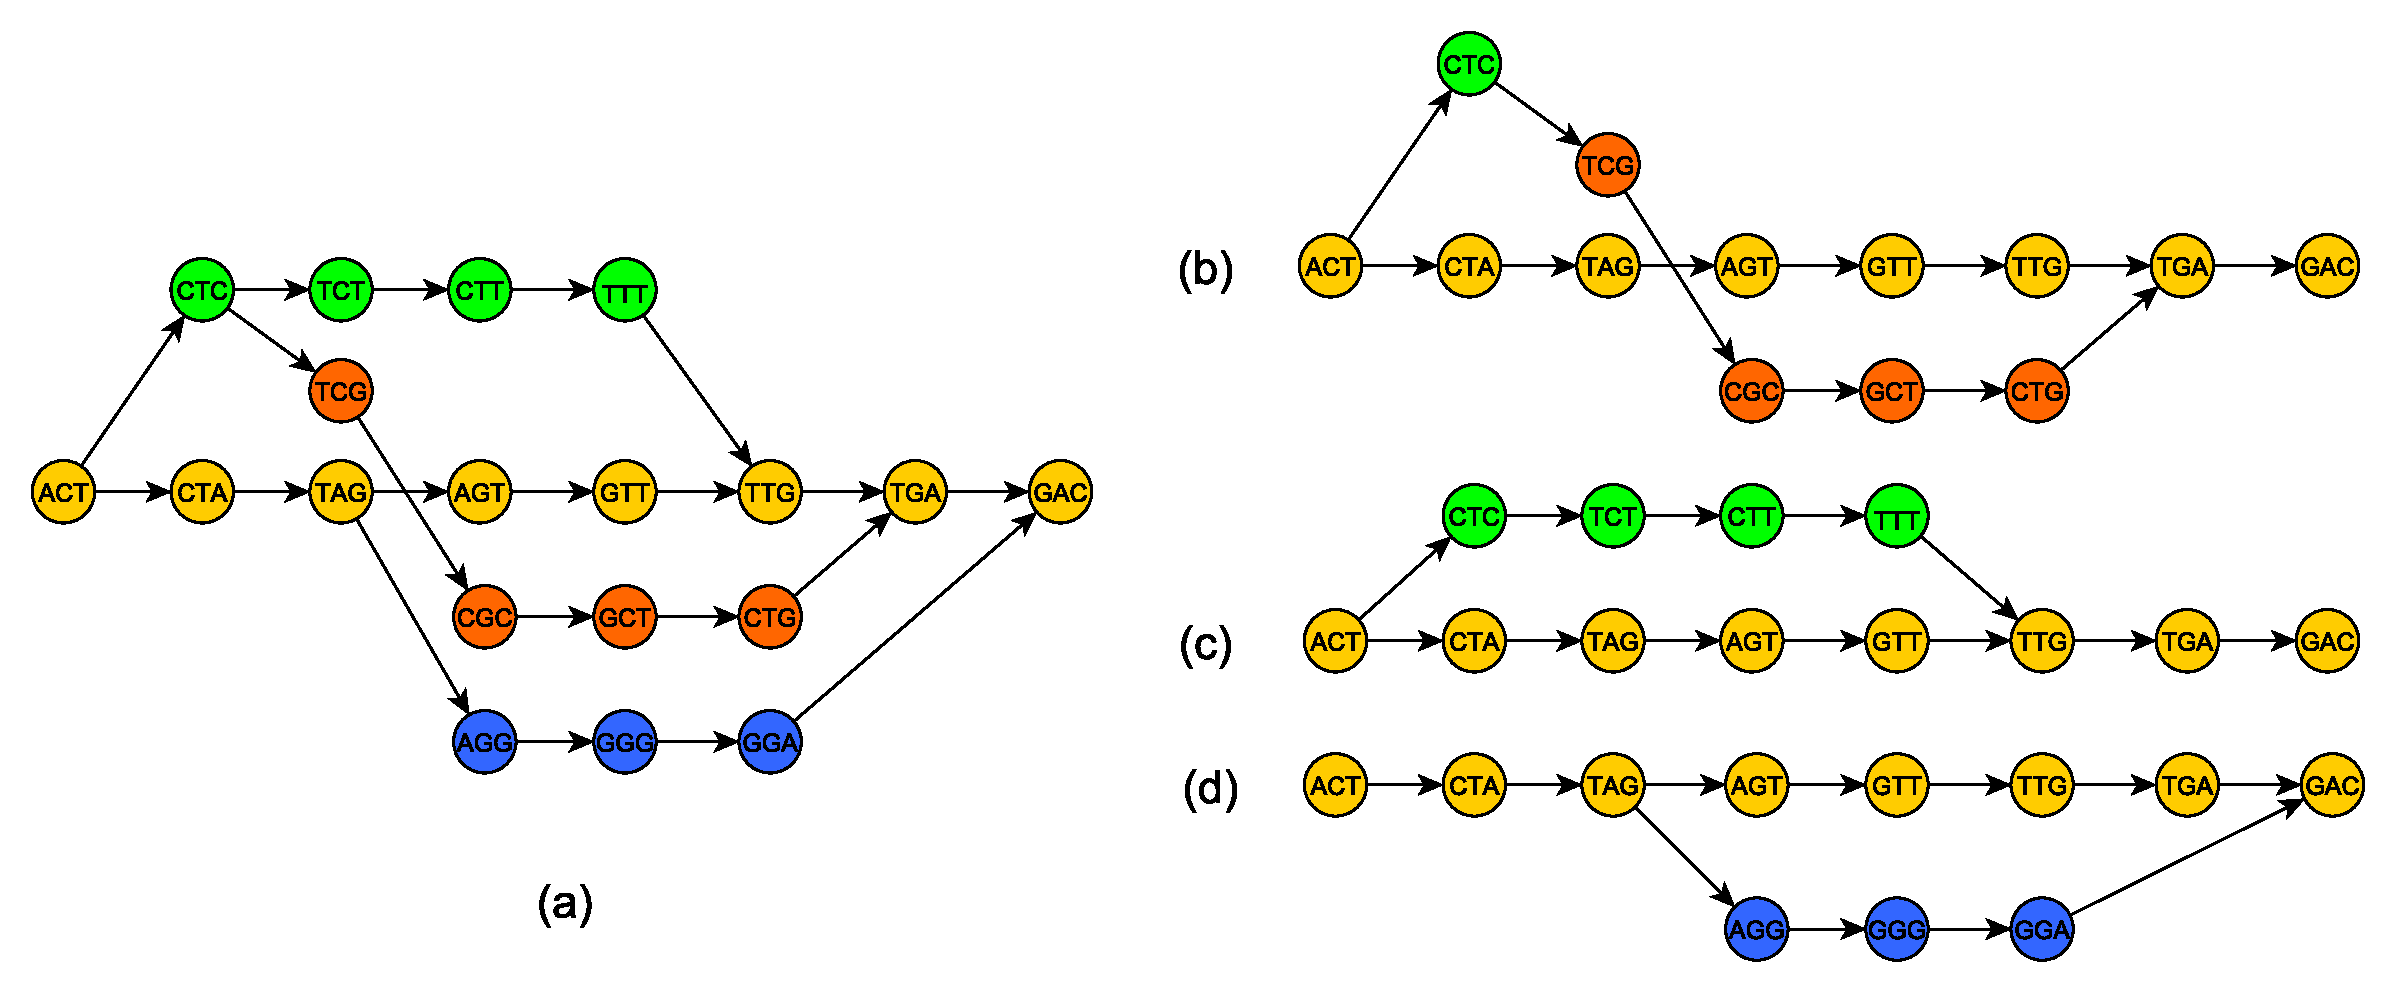
\includegraphics[width=\textwidth]{img/cv_ex.pdf}
	\caption{Пузыри, образованные сложными геномными вариациями: (a) подграф, содержащий пути, соответсвующие гомологичным последовательностям; (b) пузырь, образованный двумя заменами нуклеотидов в последовательных к-мерах; (c) пузырь, образованный двумя заменами нуклеотидов в одном к-мере; (d) пузырь, образованный комбинацией замены и удаления нуклеотидов.}
	\label{fig:cv_ex}
\end{figure*}

Заметим, что сложный пузырь может быть поставлен в соответсвие последовательности простых пузырей, каждый из которых относится к точечной мутации, как показано на рисунке \ref{fig:pm_to_cv}. Таким образом, количество точечных мутаций между последовательностями может быть рассчитано обходом графа.
\begin{figure*}[h!t]
	\centering
	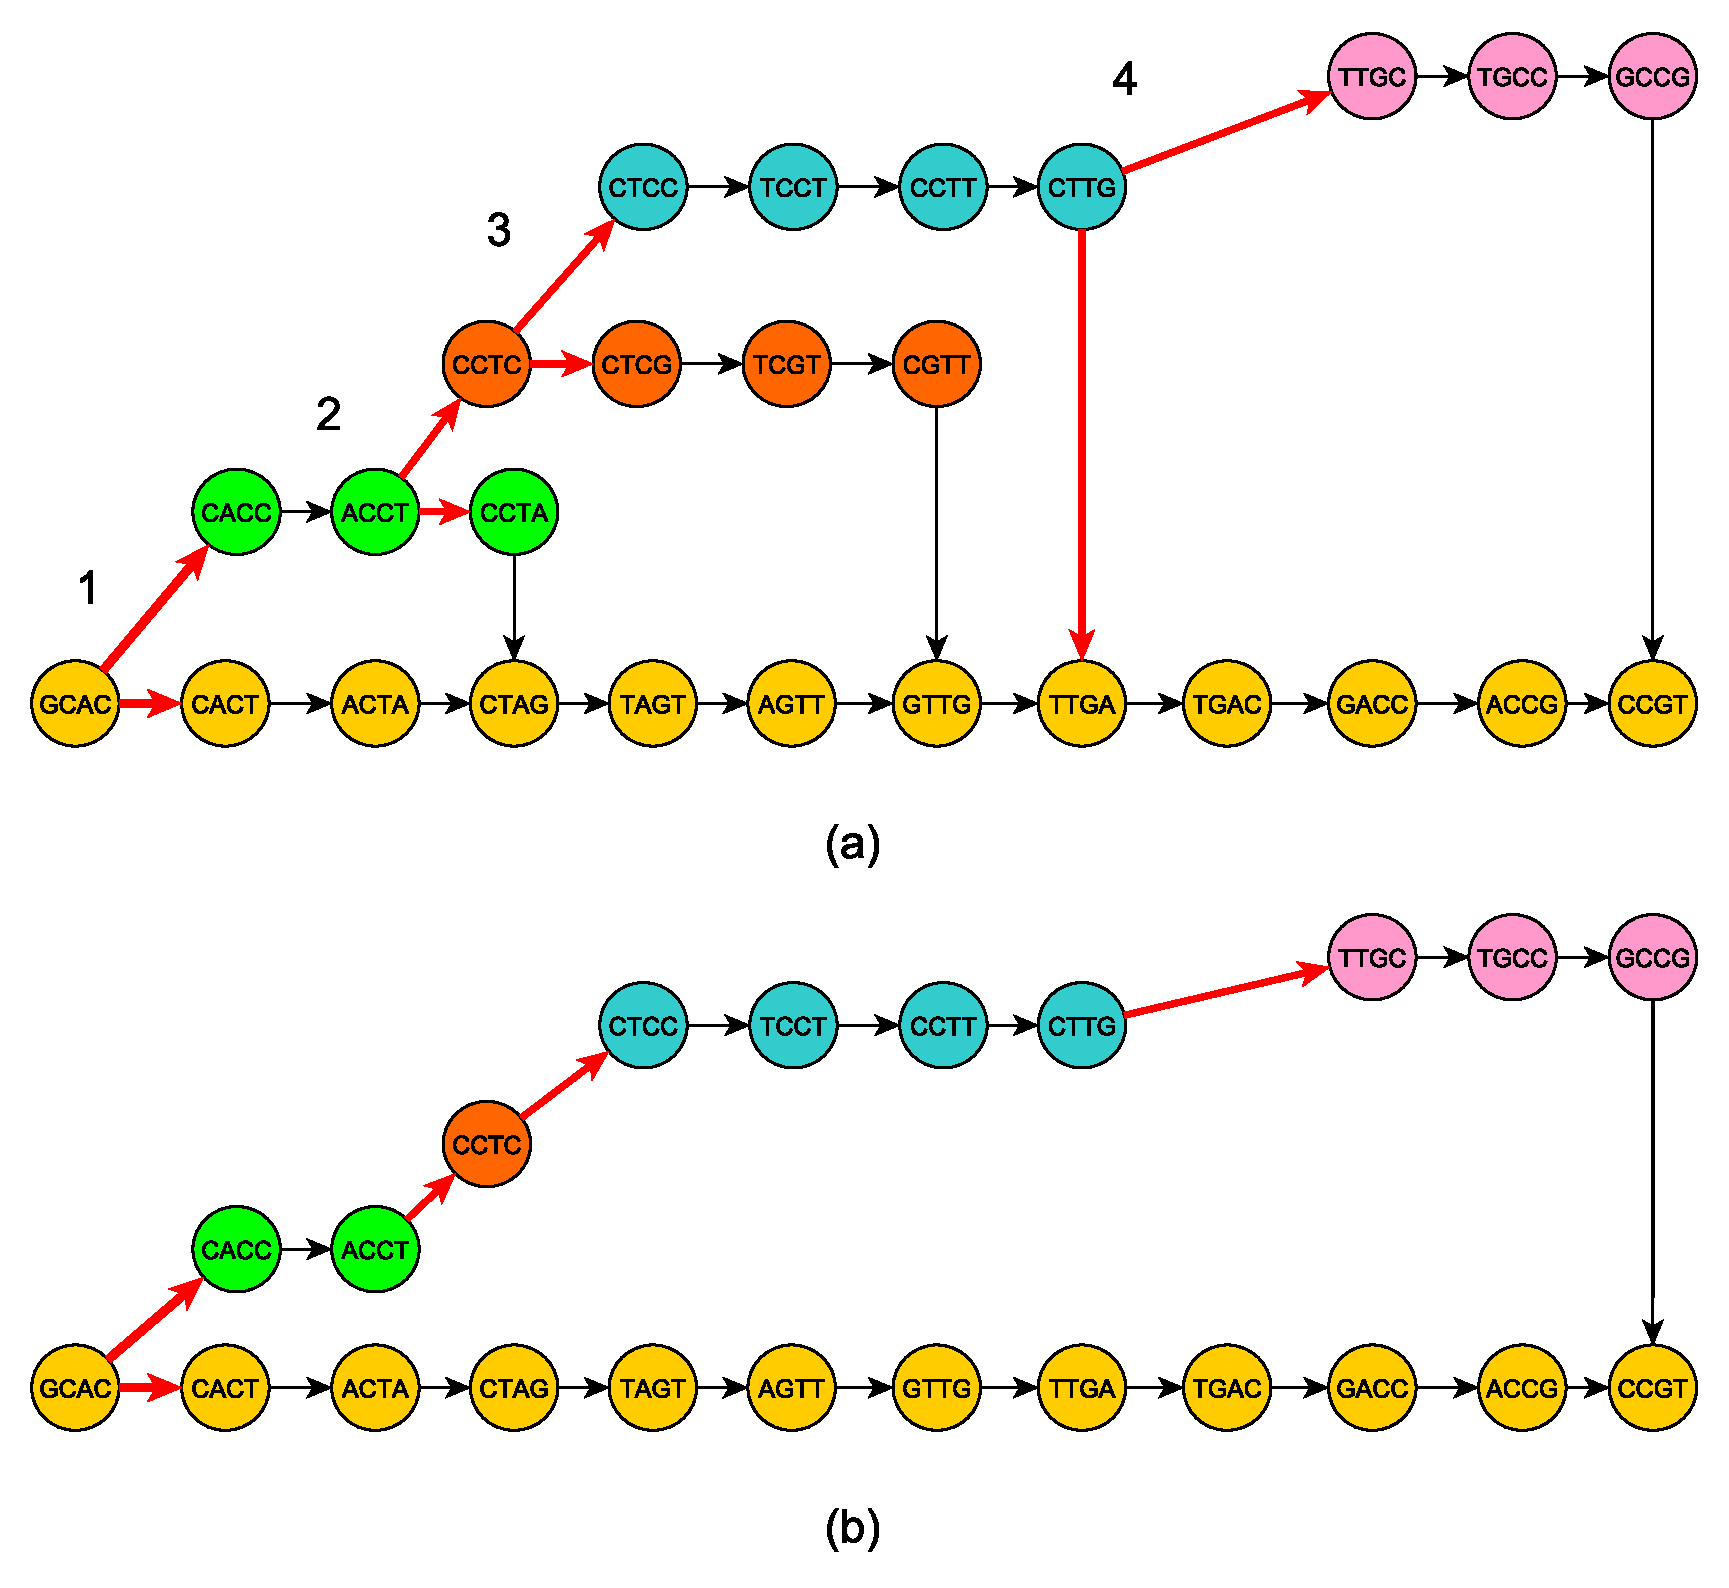
\includegraphics[width=0.7\textwidth]{img/pm_to_cv.pdf}
	\caption{Простые пузыри, составляющие сложный пузырь: (a) подграф, соответствующий нескольким точечным мутациям; (b) сложный пузырь, образованный последовательностью простых пузырей.}
	\label{fig:pm_to_cv}
\end{figure*}

\pagebreak